
\section*{1}
Lennard Jones potensialet is given by the function.
\begin{equation}
U(r) = 4\epsilon \left(   (\frac{\sigma}{r})^{12} -   (\frac{\sigma}{r})^6 \right)
\end{equation}

\subsection*{i}
Plot the potential as a function of r with $\epsilon$ = 1 and $\sigma$ = 1, for \textbf{example for $r \in [0.9, 3]$}
\begin{figure}[h!]
        \centering 
        %Scale angir størrelsen på bildet. Bildefilen må ligge i samme mappe som tex-filen. 
        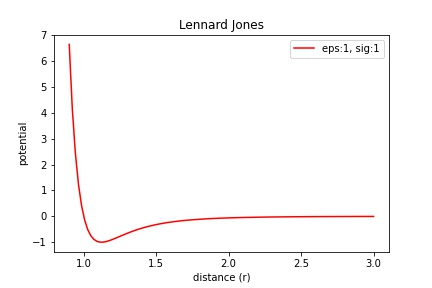
\includegraphics[scale=0.6]{1a_i.jpg} 
        \caption{Lennard Jones potential with $\epsilon = 1$ and $\sigma = 1$, }
        %Label gjør det enkelt å referere til ulike bilder.
        \label{fig:eksempelbilde1}
\end{figure}

\subsection*{ii}

The term in the twelfth power $\frac{\sigma}{r}^12$ dominates for $r < \sigma$ because the powered term is $ > 1$. The high power means the value of the first term blows up quickly. When $r < \sigma$, it will be quickly diminished. When $r = \sigma$ the two terms cancel out. The effect is that for values at distance where $r > \sigma$, there is an attractive force and for $r < \sigma$ a repelled force.

\subsection*{iii}
The equillibrium points can be identified by looking at the graph. For what values of $r$ cannot the bonding potential be increased by altering the distance. This must be where the derivative of the potential is 0, which happens at approximately $r = 1.1\sigma$. 

\subsection*{iv}
The motion of two atoms starting at terst separated by distance of *$1.5 \sigma$ (i.e if the $\sigma$ is 1, then $r = 1.5$  will be subject to a weak negative gradient. This attraction will grow until it reaches the maximum bonding potential at around radius of $r = 1.1 \sigma$.
If the particles in stead start at 0.95, they will move away from one another and again stabilize at the same point of maximum bonding potential.

\subsection*{v}
Around the point of maximum bonding potential, the potential can be approximated by a parabolic equation, such as $x^2$. There are other forces that act in this way, including the weak and the strong nuclear force.

\section*{1b)}

\subsection*{i}
The force acting atom $i$ at position $\vec{r_i}$ from atom $j$ at position $r_j$ must then be:

\begin{equation}
U(r) = 4\epsilon \left(   (\frac{\sigma}{| r_i - r_j | })^{12} -   (\frac{\sigma}{| r_i - r_j | })^6 \right)
\end{equation}

\subsection*{ii}
TODO : Show that the equation of motion:


The key to understand this is at the potential is accelerating an object, which means it is impacting the second derivative of an equation whic tracks the position of an atom.

If we start with an unknown equation for motion, we know that the change in motion is given by $|| \vec{r_i}  - | \vec{r_j}  | $. 

\begin{equation}
\vec{r_i} = f(\vec{r_i}, \vec{r_i}')
\end{equation}


The force acting on a given particle must then be the sum of all the vector-forces acting on the particle, which in theory are the force from all the other particles except itself. The $k \neq i$ ensures that we do not count any forces acting on itself

\begin{equation}
  \sum_{j \neq i} 4\epsilon \left(   (\frac{\sigma}{| r_i - r_j | })^{12} -   (\frac{\sigma}{| r_i - r_j | })^6 \right)
\end{equation}

With $\sigma = 1$, this can be rewritten to:

\begin{equation}
  \sum_{j \neq i} 4\epsilon \left(   | r_i - r_j |^{-12} -   (| r_i - r_j |^{-6} \right)
\end{equation}

Acceleration is the second derivative of the position. The expression we are looking at is therefore the second derivative of the position. In reality. If we define the middle term $u = \left(   | r_i - r_j |^{-12} -   (| r_i - r_j |^{-6} \right) $, we can see. 


\begin{equation}
\int  u du  = \frac{1}{2} u^2 \frac{1}{u'}
\end{equation}

Derivating again we get:
\begin{equation}
\int  u du  = \frac{1}{6} u^3 \frac{1}{u'^2}
\end{equation}

However, the force of the potential, like all other forces become weaker with the square of the distance. So we must also weaken the potential by multiplying with the the distance divided by the square of the distance $ (\frac{\sigma}{| r_i - r_j | })$ T
\begin{equation}
  \sum_{j \neq i} 4\epsilon \left(   | r_i - r_j |^{-12} -   (| r_i - r_j |^{-6} \right) (\frac{\vec{r_i} - \vec{r_j}}{| r_i - r_j |^2}) 
\end{equation}


\subsection*{1c)}
Using reduces units, this simplifies calculations considerably. We have modified the acceleration equation so that the distance between atoms is measured in sigmas $\sigma$. The result of this is that the equation :

\begin{equation}
  \sum_{j \neq i} 4\epsilon \left(   (\frac{\sigma}{| r_i - r_j | })^{12} -   (\frac{\sigma}{| r_i - r_j | })^6 \right)
\end{equation}

are converted into 

\begin{equation}
  \sum_{j \neq i} 4\epsilon \left(   (\frac{1}{| r_i - r_j | })^{12} -   (\frac{1}{| r_i - r_j | })^6 \right)
\end{equation}

\subsection*{ii}
TODO : What is the characteristic time-scale?

We have $\sigma = 3.405 Å, Å = 10*{-10}meters,  m = 39.95 u, u = 1.66 \cdot 10*{-27}, \epsilon = 1.0318 \cdot 10^2 ev,  ev = 1.602 10^-{19}$


\subsection*{iii}

